\documentclass[12pt, letterpaper]{article}
\usepackage[titletoc,title]{appendix}
\usepackage{color}
\usepackage{booktabs}
\usepackage[usenames,dvipsnames,svgnames,table]{xcolor}
\definecolor{dark-red}{rgb}{0.75,0.10,0.10}
\definecolor{bluish}{rgb}{0.05,0.05,0.85}

\usepackage[margin=1in]{geometry}
\usepackage[linkcolor=blue,
			colorlinks=true,
			urlcolor=blue,
			pdfstartview={XYZ null null 1.00},
			pdfpagemode=UseNone,
			citecolor={bluish},
			pdftitle={pareto_party}]{hyperref}

\usepackage[resetlabels,labeled]{multibib}
\newcites{SI}{SI References}
\usepackage{natbib}

\usepackage{float}

\usepackage{geometry} % see geometry.pdf on how to lay out the page. There's lots.
\geometry{letterpaper}               % This is 8.5x11 paper. Options are a4paper or a5paper or other... 
\usepackage{graphicx}                % Handles inclusion of major graphics formats and allows use of 
\usepackage{amsfonts,amssymb,amsbsy}
\usepackage{amsxtra}
\usepackage{verbatim}
\setcitestyle{round,semicolon,aysep={},yysep={;}}
\usepackage{setspace}		     % Permits line spacing control. Options are \doublespacing, \onehalfspace
\usepackage{sectsty}		     % Permits control of section header styles
\usepackage{pdflscape}
\usepackage{fancyhdr}		     % Permits header customization. See header section below.
\usepackage{url}                     % Correctly formats URLs with the \url{} tag
\usepackage{fullpage}		%1-inch margins
\usepackage{multirow}
\usepackage{rotating}
\setlength{\parindent}{3em}

\usepackage[T1]{fontenc}
\usepackage[bitstream-charter]{mathdesign}

\usepackage{chngcntr}
\usepackage{booktabs}
\usepackage{longtable}

\def\citeapos#1{\citeauthor{#1}'s (\citeyear{#1})}

\makeatother

\usepackage{footmisc}
\setlength{\footnotesep}{\baselineskip}
\makeatother
\renewcommand{\footnotelayout}{\normalsize \doublespacing}


% Caption
\usepackage[hang, font=small,skip=0pt, labelfont={bf}]{caption}
%\captionsetup[subtable]{font=small,skip=0pt}
\usepackage{subcaption}

% tt font issues
% \renewcommand*{\ttdefault}{qcr}
\renewcommand{\ttdefault}{pcr}

\setcounter{page}{0}

\usepackage{lscape}
\renewcommand{\textfraction}{0}
\renewcommand{\topfraction}{0.95}
\renewcommand{\bottomfraction}{0.95}
\renewcommand{\floatpagefraction}{0.40}
\setcounter{totalnumber}{5}
\makeatletter
\providecommand\phantomcaption{\caption@refstepcounter\@captype}
\makeatother

\title{Partisan Vision? Do Partisans See Differently?}

\author{Gaurav Sood\thanks{Gaurav can be reached at, \href{mailto:gsood07@gmail.com}{\texttt{gsood07@gmail.com}}} \and Alex Theodiridis\thanks{Alex can be reached at \href{alexandertheodoridis@gmail.com}{\texttt{alexandertheodoridis@gmail.com}}}}


\begin{comment}

setwd(paste0(githubdir, "partisan_vision/ms/"))
tools::texi2dvi("partisan_vision.tex", pdf = TRUE, clean = TRUE)
setwd(githubdir)

\end{comment}

\begin{document}
\maketitle
\thispagestyle{empty}

\begin{abstract}

\noindent In the current era of partisan polarization, there is concern that partisanship that strongly colors partisans' worldview. But does it cause us to \textit{see} things differently \citep{chabris2010invisible}? We test the hypotheses in three different experiments and consistently find that the effect is at worst small.
\end{abstract}

\newpage

\doublespacing

Partisans are increasingly polarized \cite{IyengarSoodLelkes2012} with partisan cleavages outstripping some of the longer standing racial cleavages. 

In this paper, we explore whether polarization affects . We test this with some simple evaluative tasks---finding errors---with subtle cues about party.

\section{Data and Research Design}

\citep{chabris2010invisible}

To assess how partisans `see', we surveyed a nationally representative sample of people selected by YouGov \citep{rivers2007} as part of a Cooperative Congressional Election Study (CCES) module. We conducted two experiments. In the first experiment, we changed one single word (democratic/republican) to change who respondents thought wrote a piece of text (see Figure~\ref{fig:mistakes_dem} and Republicans \ref{fig:mistakes_rep}). We then asked ``How many errors did you count?''

In the second survey, we showed people a photo of a parking lot and asked them to estimate the number of poorly parked cars. We manipulated which party's members were using the parking lot. 

On a survey on M-Turk, we asked respondents to watch a short video and estimate how many people in the video were wearing masks. In particular, our directions were as follows:

``Please watch the following short (10-second) video. You will be asked a question about it on the next screen. ...How many people in the video were wearing masks?''

\section{Results}

As Table~\ref{tab:tab1} shows, Democrats find 9.7 mistakes when they think the text is written by a Democrat compared to 9.9 mistakes when they think the text is written by a Republican. On the other hand, Republicans find 8.4 mistakes on average when they think the text is written by a Democrat and 8.1 mistakes when they think it is written by a Republican. And while the differences are consistent with the point about partisan bias, the main point is about the smallness of the differences. 


\begin{figure}[!htbp]
\centering
\caption{Poorly Parked Cars}
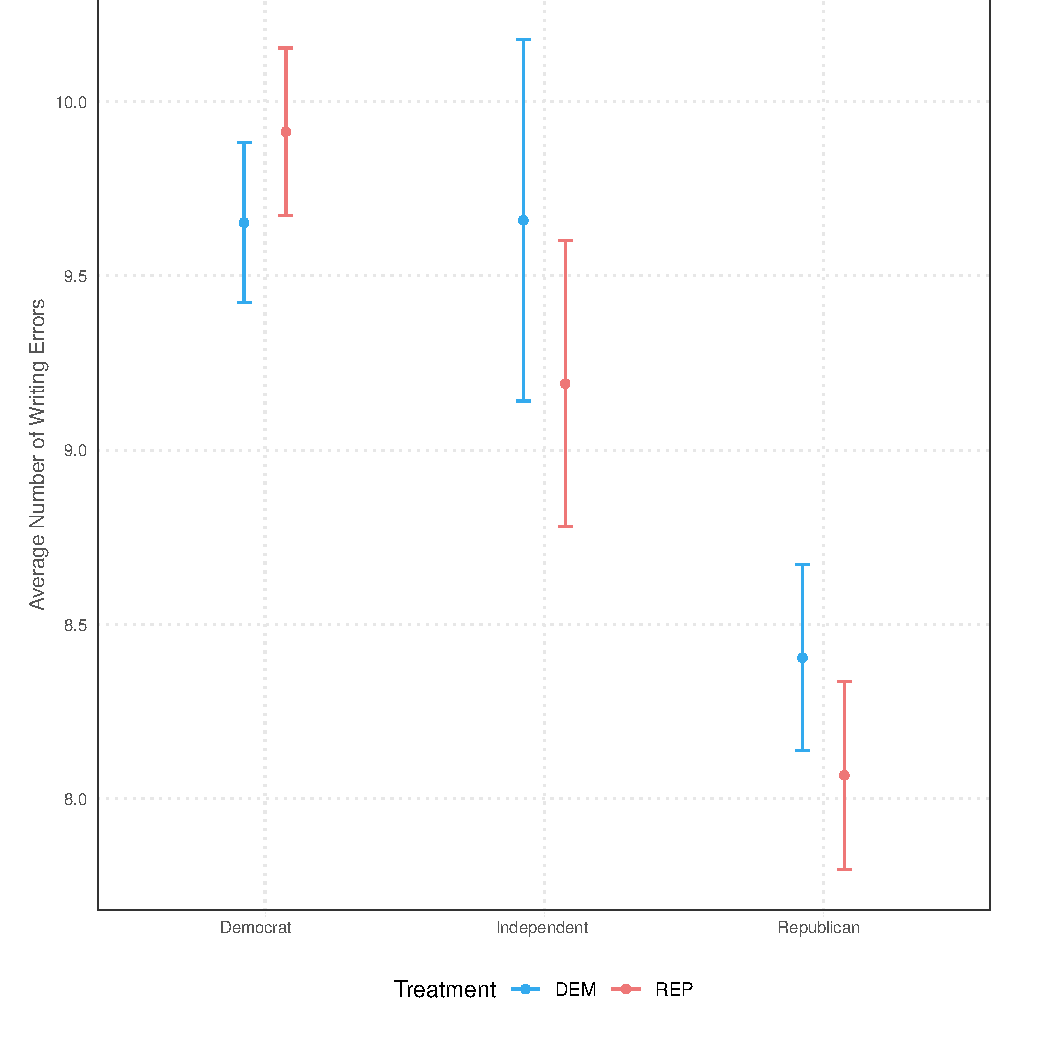
\includegraphics[scale=.6]{../figs/error.pdf}
\label{fig:mistakes_rep}
\end{figure}


\begin{figure}[!htbp]
\centering
\caption{Poorly Parked Cars}
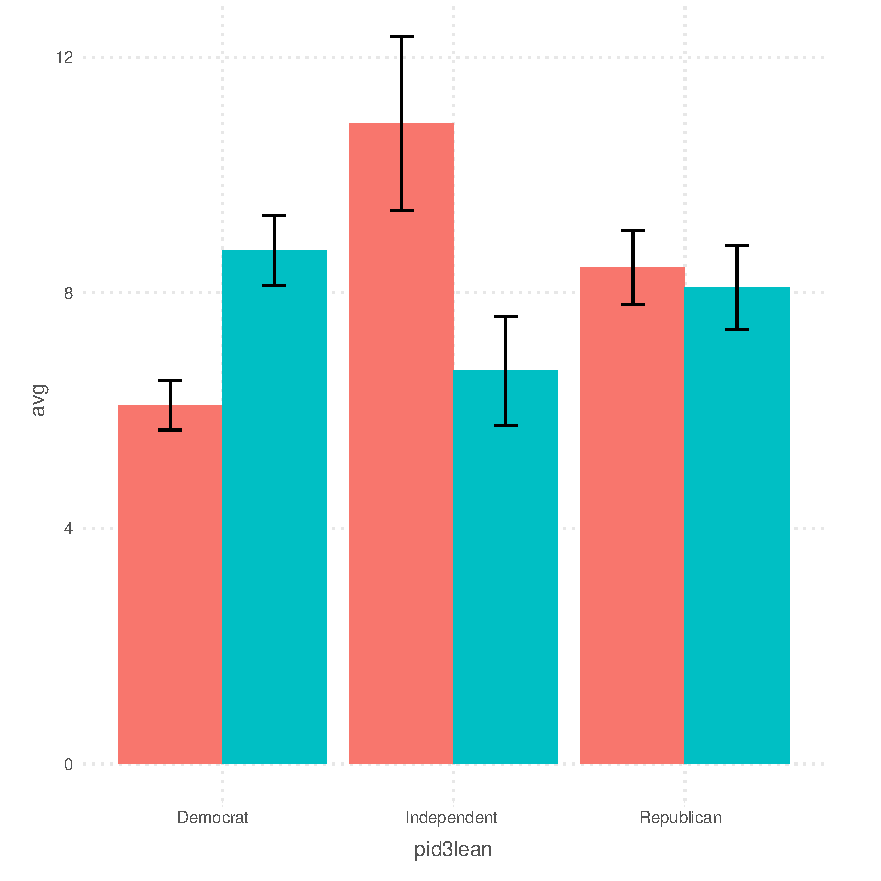
\includegraphics[scale=.6]{../figs/parking.pdf}
\label{fig:mistakes_rep}
\end{figure}


\clearpage
\bibliographystyle{apsr}
\bibliography{vision}
\clearpage


\appendix
\renewcommand{\thesection}{SI \arabic{section}}
\setcounter{table}{0}\renewcommand\thetable{\thesection.\arabic{table}}  
\setcounter{figure}{0}\renewcommand\thefigure{\thesection.\arabic{figure}}
\counterwithin{figure}{section}

\section{Figures}
\begin{figure}[!htbp]
\centering
\caption{Share of Black Criminals in Law \& Order and the Real World}
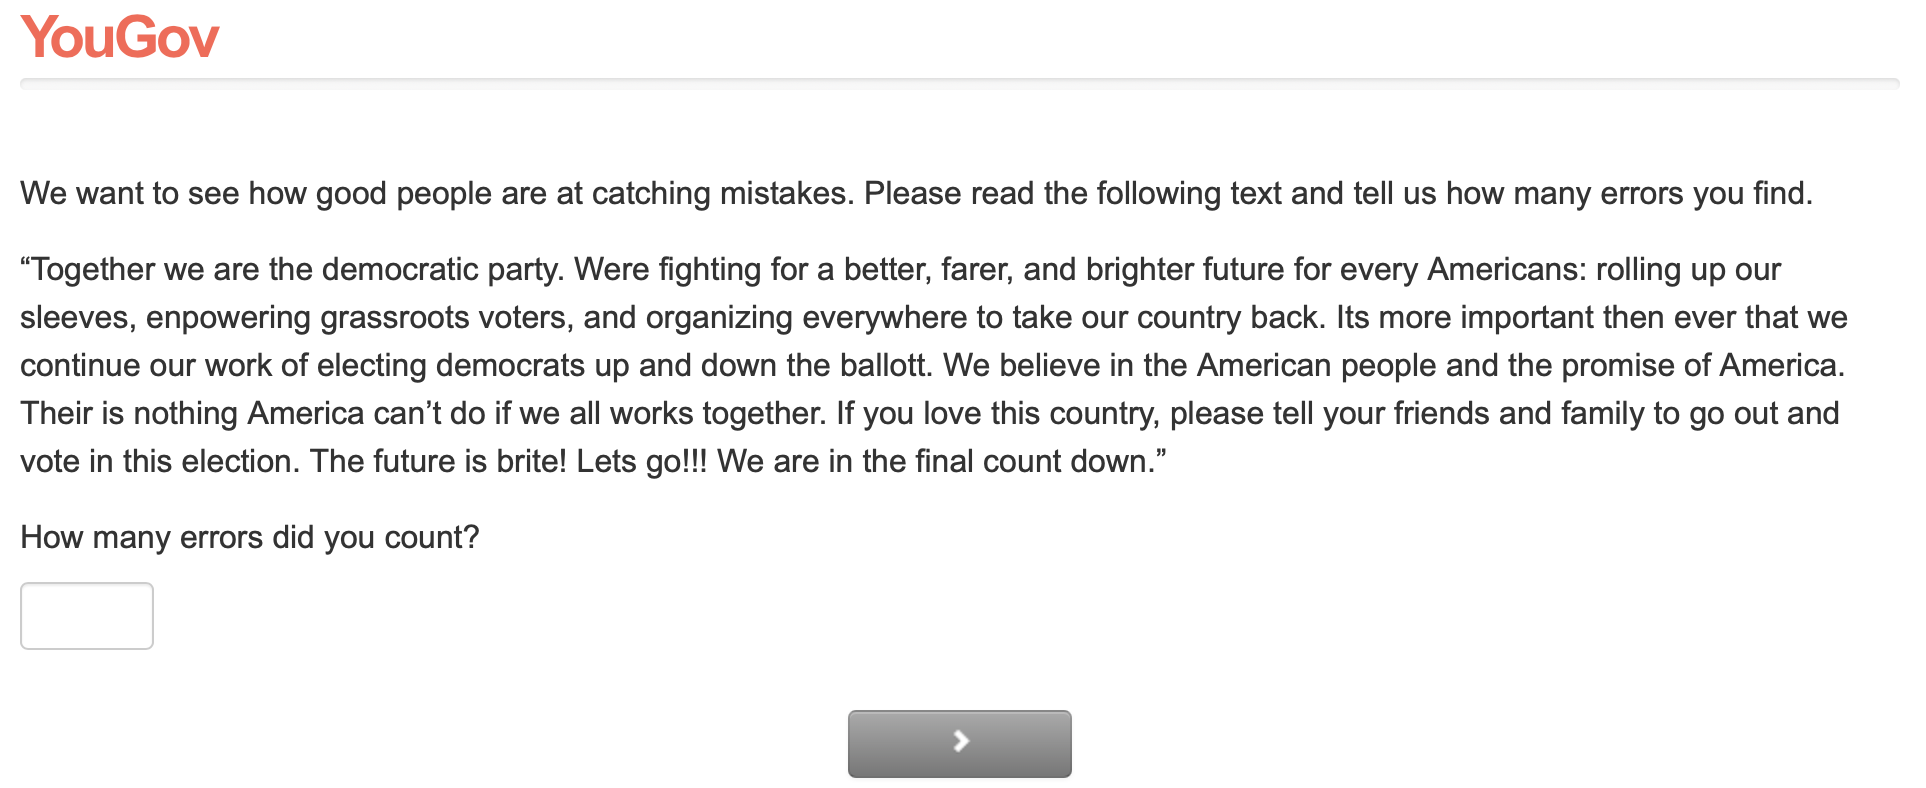
\includegraphics[scale=.4]{../data/treats/Mistakes_Dem.png}
\label{fig:mistakes_dem}
\end{figure}

\begin{figure}[!htbp]
\centering
\caption{Mistakes}
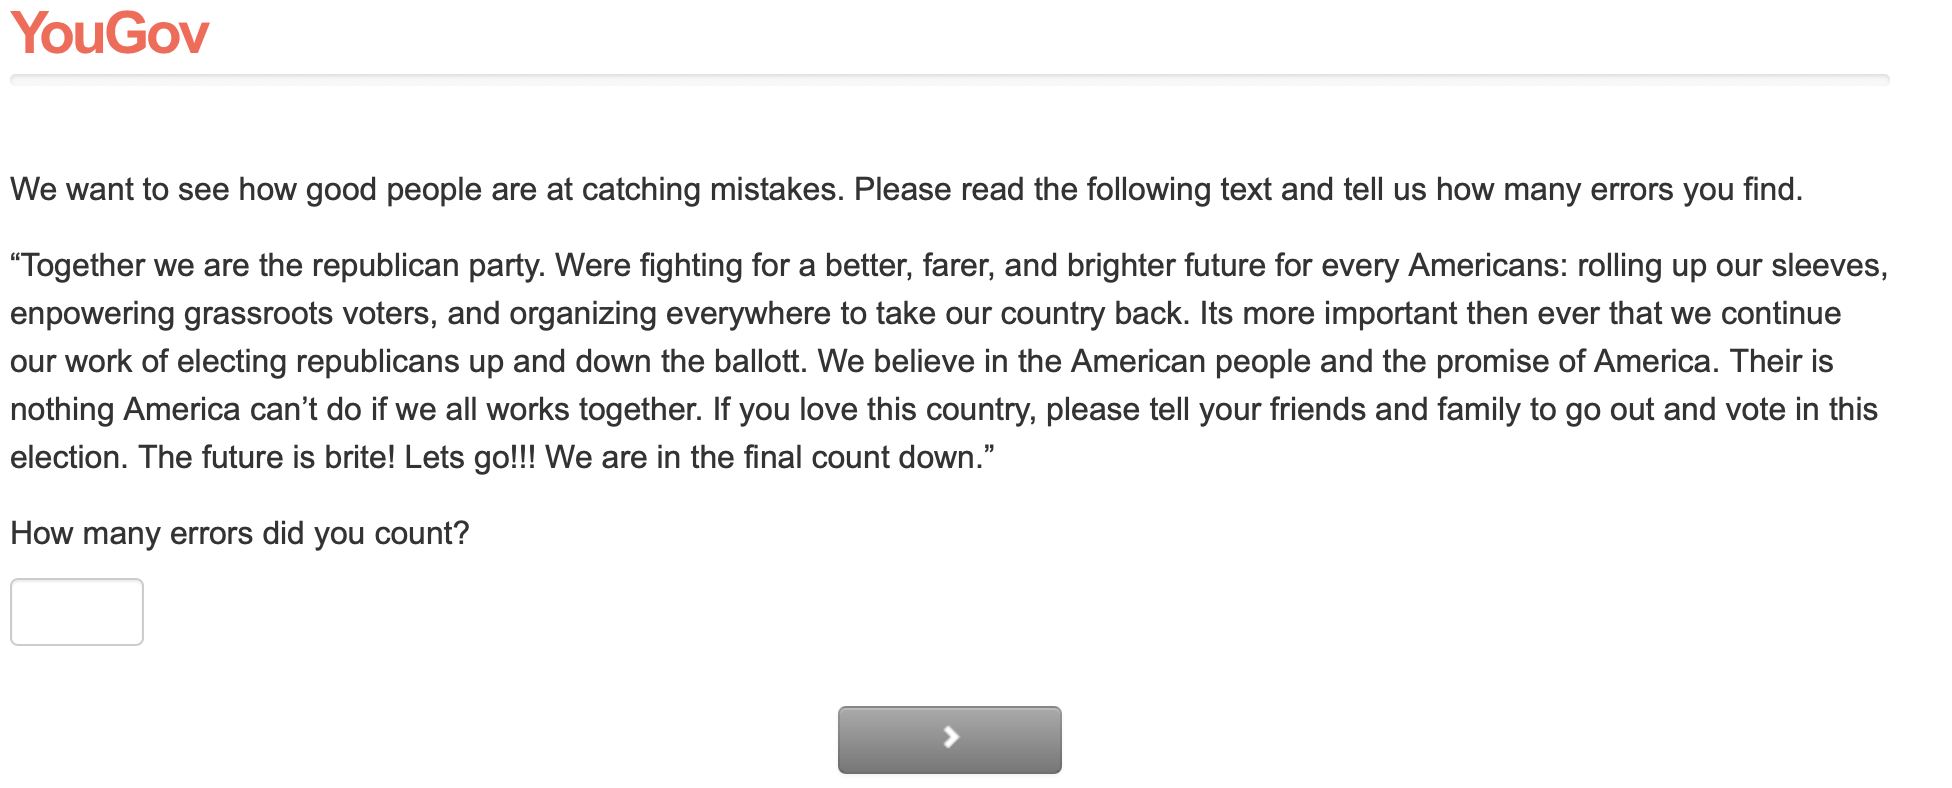
\includegraphics[scale=.4]{../data/treats/Mistakes_Rep.png}
\label{fig:mistakes_rep}
\end{figure}

\begin{figure}[!htbp]
\centering
\caption{Parking Lot}
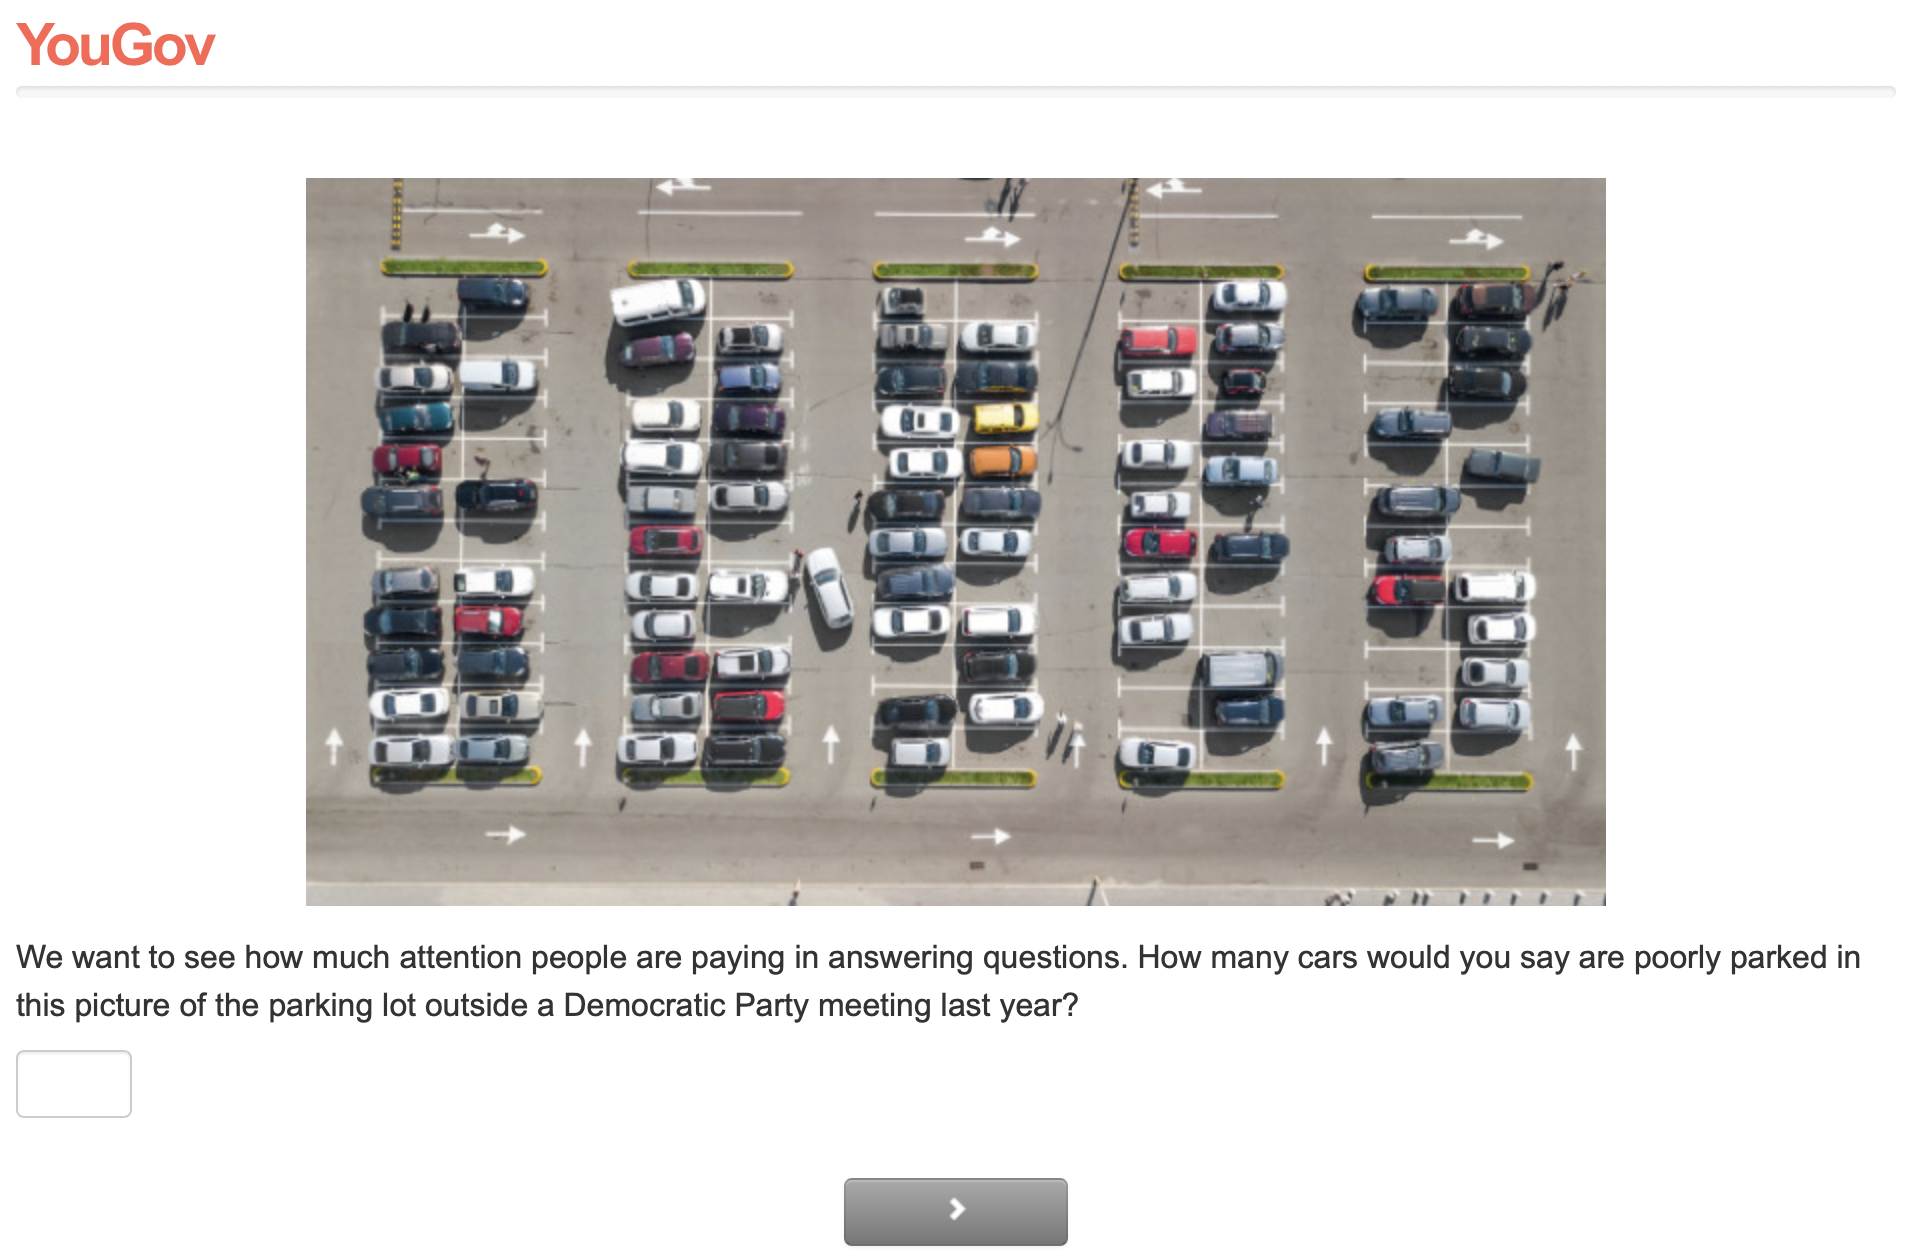
\includegraphics[scale=.4]{../data/treats/Parking_Lot_Dems.png}
\label{fig:mistakes_rep}
\end{figure}

\clearpage
\section{Tables}
% latex table generated in R 4.2.2 by xtable 1.8-4 package
% Sun Nov 27 20:42:19 2022
\begin{table}[!htb]
\centering
\caption{Average Number of Writing Errors} 
\label{tab:error_sum}
\begin{tabular}{llrrrr}
  \hline
pid3lean & Error\_split & avg & med & n & std\_error \\ 
  \hline
Democrat     & DEM & 9.7 & 10.0 & 334 & 0.2 \\ 
  Democrat     & REP & 9.9 & 10.0 & 324 & 0.2 \\ 
  Independent  & DEM & 9.7 & 10.0 & 94 & 0.5 \\ 
  Independent  & REP & 9.2 & 9.0 & 110 & 0.4 \\ 
  Republican   & DEM & 8.4 & 8.0 & 253 & 0.3 \\ 
  Republican   & REP & 8.1 & 8.0 & 252 & 0.3 \\ 
   \hline
\end{tabular}
\end{table}

% latex table generated in R 4.1.2 by xtable 1.8-4 package
% Sun Nov 14 23:57:16 2021
\begin{table}[!htb]
\centering
\begin{tabular}{llrrr}
  \hline
pid3lean & UCMParking\_split & avg & med & n \\ 
  \hline
Democrat     & Democratic Party & 6.1 & 5.0 & 211 \\ 
  Democrat     & Republican Party & 8.7 & 6.0 & 212 \\ 
  Independent  & Democratic Party & 10.9 & 7.0 & 57 \\ 
  Independent  & Republican Party & 6.7 & 5.0 & 61 \\ 
  Republican   & Democratic Party & 8.4 & 6.0 & 181 \\ 
  Republican   & Republican Party & 8.1 & 5.0 & 163 \\ 
   \hline
\end{tabular}
\caption{Average Number of Errors} 
\label{tab:error_sum}
\end{table}


\end{document}